\begin{section}{Organizers}
	\label{sec:organizer}
	When the organizer is succesfully signed in, he will be redirected to his dashboard.
	The organizer also has the default user functionalities that have been previously
	mentioned. But he will also be some extra links presented that are exclusively
	available to organizers.
	
	\begin{subsection}{Manage Pupils}
		\label{sec:organizer_manage_pupils}
		Upon entering this page, there will be a table visible with all the (basic) users
		registered in the Bebras application. Columns include but are not limited to:
		\begin{itemize}
			\item Bebras-ID
			\item Name
			\item Email Address
			\item Class, [School]
			\item Gender
			\item Age
			\item Actions
		\end{itemize}
		The actions column contains multiple buttons that can perform different actions
		for each user, these actions are the following:
		\begin{itemize}
			\item Delete
			\item Edit
			\item Block
			\item Mimic
			\item History
		\end{itemize}
		There is also one Add button at the top of the page. After clicking it, the
		organizer will be redirected to a page identical to
		\nameref{sec:organizer_edit_pupils}, with the only difference that no fields
		are filled in. The history button will open a new page that shows a list of all
		the previous ClassGroups that the Pupil was part of in the past. \\
		\\
		The multi-actions in this form are the following:
		\begin{itemize}
			\item Delete
			\item Edit ClassGroup
			\item Block
		\end{itemize}
		The first action will simply remove the selected pupils, but the other actions
		redirect the organizer to edit pages identical to their single-edit equivalent.
		\begin{subsubsection}{Delete Pupils}
			When the organizer whishes to remove a pupil, he can click on the delete
			button in the row of that user. A confirmation dialog will be shown after
			clicking it, to make sure the organizer really wants to delete that user. \\
			The user will not really be deleted from the database, but only unlinked so
			that the statistics are in no way harmed.
		\end{subsubsection}
		\begin{subsubsection}{Edit Pupils}
			\label{sec:organizer_edit_pupils}
			The Edit button will redirect the user to a dedicated edit-screen where all
			the fields of a pupil that are available in the database are presented in a
			form and can be modified. Every field of the form is a regular text-field.
			Upon saving the form by clicking the button on the bottom of the form, the
			form will be checked and the organizer will be notified if there are errors
			in the form and where they are. For example a non-existing ClassGroup ID.
			When there were no errors while editing, the organizer will be redirected to
			the main pupil-management page.
		\end{subsubsection}
		\begin{subsubsection}{Block Pupils}
			\label{sec:organizer_block_pupils}
			When pupils are misbehaving, the organizer has an option to temporarily or
			permanently block an user from the application. When the organizer clicks on
			the Block button, he will be redirected to a new page where he will be presented
			to a small form where he has the choice to select not-blocked, permanent or
			temporarily. When he chooses temporarily, a new input box will become visible
			where he can choose the date for when the user should become active again.
			When a user is already being blocked,
			the organizer is able to visit this screen and change the current
			blocking-mode.
		\end{subsubsection}
		\begin{subsubsection}{Mimic Pupils}
			Upon pressing this button, the organizer will be redirected to the dashboard
			of the selected pupil. He will be able to do anything that pupil can, and
			nothing else. Only when the disguised organizer clicks on the log-out button,
			he will be redirected to the page he left off, in this case the Pupil
			management.
		\end{subsubsection}
		
	\end{subsection}
	
	\begin{subsection}{Manage Teachers}
		The Teacher management page is identical to the Pupil management page, with the
		only difference that there is also a phone-number field that is only available
		to the teacher.
	\end{subsection}
	
	\begin{subsection}{Manage ClassGroups}
		This page is identical to the ClassGroup management page that is available to the
		teachers, but the organizers are able to see all the available classgroups that
		are present in the application. The organizer is also able to change the ownership
		of the class to another teacher in the Edit ClassGroup form.
	\end{subsection}
	
	\begin{subsection}{Manage Questions}
		This page contains two tables that are positioned next to each other. \\
		The first table contains all the servers that provide the hosting of questions.
		This is nothing more than a simple list of names of the server, base-url and
		optional additional path to the questions base folder. \\
		The second table contains all the questions and has the following columns:
		\begin{itemize}
			\item ID
			\item Server
			\item Official/Regular
			\item Active
		\end{itemize}
		The Server's field contains the name of a certain server specified in the first
		table and the ID is the name of a subfolder on that server that contains all the
		resource files necessary for that question.
		The last two fields are simple toggles that say whether the question is official
		or regular and whether the question is active or not. Non-active questions are
		not usable in the rest of the application, they can be useful when a question
		needs evaluation or is not yet fully finished. \\
		\\
		This table also have Add buttons at the top, and Edit and Delete buttons in each
		row that perform equivalent actions as in \nameref{sec:organizer_manage_pupils}.
		\\
		\\
		Each row in the questions table also have select boxes that are needed to perform
		the following multi-actions:
		\begin{itemize}
			\item Change server
			\item Set official question
			\item Set regular question
			\item Activate
			\item Deactivate
		\end{itemize}
		The first multi-action will redirect the user to a simple form page where he can
		select a server for the selected questions. The other actions are simple
		toggles.\\
		\\
		The questions table also has a first row with input fields that serves as
		search fields. The last two columns require no textual input, but are simple dropdown
		lists with the values None, Official and Regular for the first one and the
		values None, Active and Inactive for the second one.\\
		\\
		There is also an extra Read action available in the table for each question, and
		also on the creation and edit form. This action allows the organizer to preview
		the question just like the pupil would see it. It's only a view action, so the
		question is not part of a competition and therefore cannot be solved. \\
		\\
		Each row also has a link to the statistics of that question.
	\end{subsection}
	
	\begin{subsection}{Manage Question sets}
		This page contains a default management form with four columns:
		\begin{itemize}
			\item ID
			\item Name
			\item Active
			\item Competition
		\end{itemize}
		The ID is unique for each set, but that is not required for the name. The active
		field can be used for sets that are still under construction and therefore cannot
		yet be used in competition creation.\\
		\\
		This table contains the default actions like creation, editing and deletion. \\
		\\
		The create and edit form contains fields for name and whether the set is active or
		not. Next to that, it also has a list where all the questions of that set are
		visible. The list shows the ID of the question and a hyperlink to the preview
		page of that question. Official questions have a special marking. Elements in this
		list can be dragged to change the order of the questions. There is no limit for 
		the maximum amount of questions per set. \\
		On the bottom of the list, there is an extra input field where questions can be
		added by their ID, the organizer can be prompted with an error message for when
		the question ID does not exist. \\
		\\
		The Edit and Create form also have a language list similar to the question list.
		Languages can be added from a preset dropdown list. Each language that is added
		to the list will be cross-checked by the server with each question. When the
		server discovers questions that are not available in some added languages, a
		permanent warning message will be displayed for each language that contains
		untranslated questions together with a list of the question ID without the
		translation. The organizer won't be able to activate a question set with such
		warnings, but he will be able to save them. The Competition field is only visible
		here, but must be changed at the Competition management page.
		
	\end{subsection}
	
	\begin{subsection}{Manage Competitions}
		This page will show a list of all the ongoing official competitions and a seperate
		list of unrestricted competitions.
		This official list shows each name of the competition together with a live countdown.
		The page will be refreshed when one or more countdowns reach zero.
		At the bottom of the list there are links to More, History and Edit.
		The list of unrestricted competitions only have an Edit link.
		\begin{subsubsection}{More}
			\begin{figure}[!h]
			  \centering
				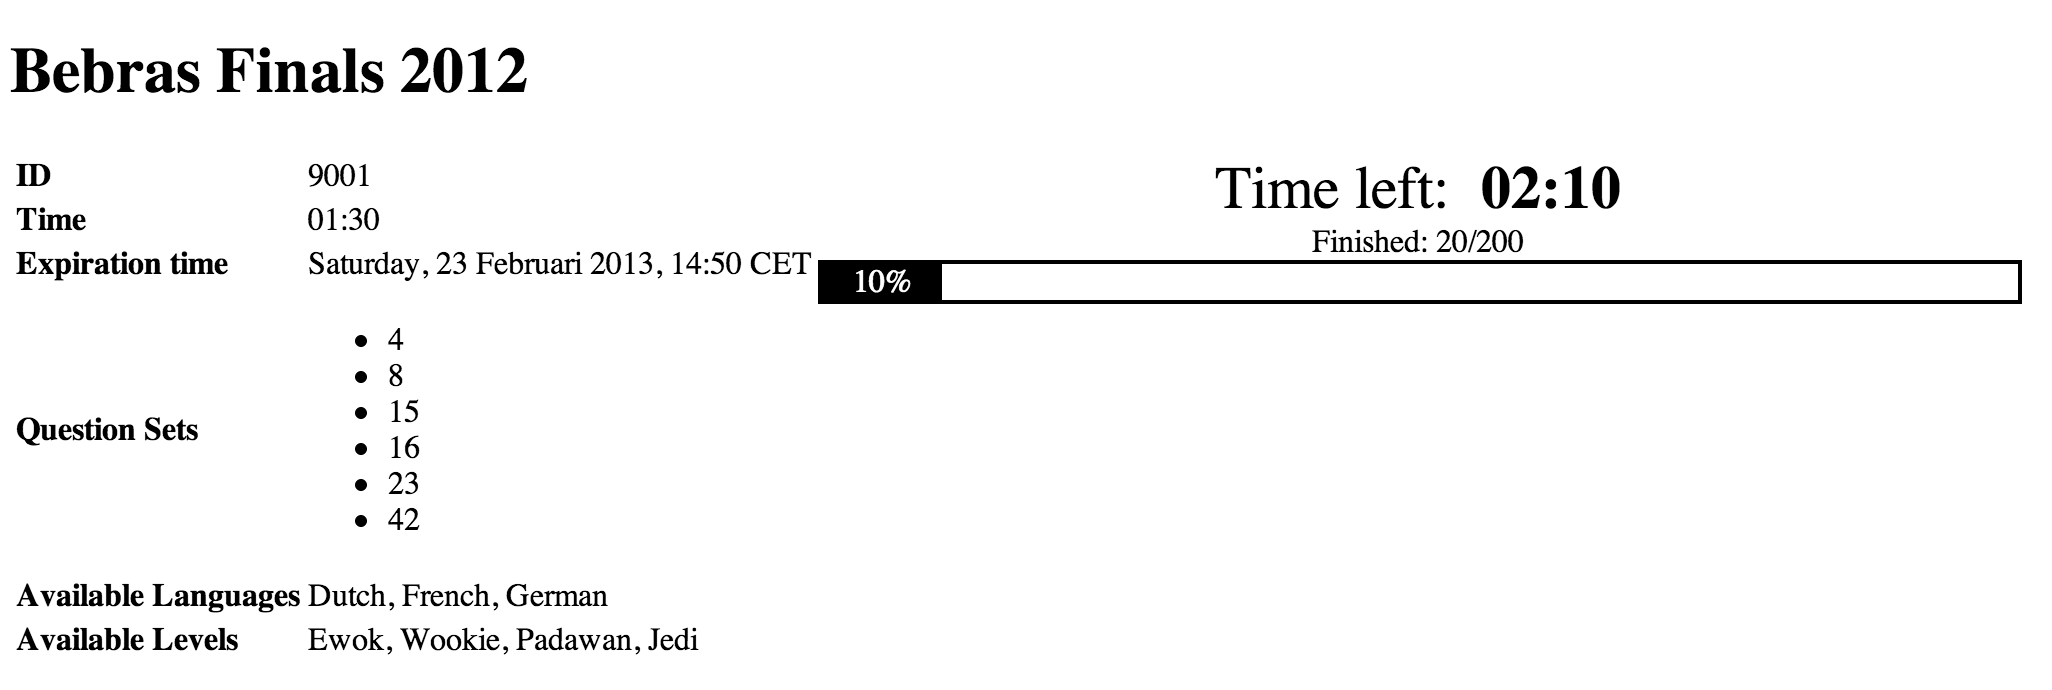
\includegraphics[width=1\textwidth]{manage_competitions_more.png}
			  \caption{More information about a running competition}
			  \label{manage_competitions_more}
			\end{figure}
			\label{sec:manage_comp_more}
			When clicking on the more link, a page will be shown with all the following
			information:
			\begin{itemize}
				\item ID
				\item Name
				\item Time
				\item Expiration time
				\item Question sets
				\item Available Languages
				\item Available Levels
				\item Registered ClassGroups
				\item Progressbar with amount of finished pupils
				\item Live countdown for expiration time
			\end{itemize}
			An example of this page can be seen in Figure~\ref{manage_competitions_more}
		\end{subsubsection}
		\begin{subsubsection}{History}
			This page will contain a simple table of finished official competitions.
			The columns are the following:
			\begin{itemize}
				\item ID
				\item Name
				\item Date finished
				\item Question sets
				\item Statistics
				\item More
			\end{itemize}
			That Statistics column contains links to the statistics for that competition and the
			Question sets column has a button that will trigger an on-page popup with a
			list of all the question sets used in that competition.\\
			\\
			The more button shows a page just like \nameref{sec:manage_comp_more}, but
			without the countdown and progressbar.
		\end{subsubsection}
		
		\begin{subsubsection}{Edit}
			This page is a default management page with the following fields:
			\begin{itemize}
				\item ID
				\item Name
				\item Time
				\item Expiration time
				\item Question sets
				\item Languages
				\item Levels
				\item Unrestricted
			\end{itemize}
			The Time field is the total amount of time each pupil gets for completing
			the competition.\\
			The expiration time is the time on which the competition will close,
			the results will be collected and the statistics will be calculated.
			Pupils won't be able to enter the competition anymore if the
			current time is larger than Expiration time - Time.\\
			The four difficulty levels are presented together with a checkbox and a
			textfield. When the checkbox is checked, that level will be available in the
			contest and a question set ID must be entered in the textfield that will be
			checked on existence upon saving.
			The Levels and Languages fields are auto-generated based on the
			available question sets. \\
			The Unrestricted field is a checkbox that defines if that competition is open
			for unrestricted quizzes. The field Expiration time is grayed out when the
			competition is unrestricted.\\
			\\
			There is an extra action Start competition that will first trigger a
			confirmation dialog and will then open the official competition after which
			the organizer will be redirected to the Competition Management page on which
			he will be able to see the ongoing competition.
		\end{subsubsection}
	\end{subsection}
	
	\begin{subsection}{Manage ClassGroups}
		This page will show two tables. One for the available classes, and one for the
		available schools.
		\begin{subsubsection}{ClassGroups}
			The ClassGroup table form has the following fields:
			\begin{itemize}
				\item ID
				\item Name
				\item Level
				\item School
				\item Teacher
			\end{itemize}
			ClassGroups can be edited by pressing their Edit action and filling in those
			fields. The School field will refer to an ID of a certain School and must
			exist just like the Teacher. Adding is similar to editing and Deleting is
			only possible if that ClassGroup contains no Pupils and has no assigned
			Teacher.
		\end{subsubsection}
		
		\begin{subsubsection}{Schools}
			The Schools table form has the following fields:
			\begin{itemize}
				\item ID
				\item Name
				\item Phone Number
				\item Address
				\item Contact Name
				\item Contact Email Address
			\end{itemize}
			This is a simple table that is only needed for the ClassGroups. Deletion of
			these Schools is only possible if no ClassGroups make use of the selected
			School.
		\end{subsubsection}
	\end{subsection}
\end{section}
